\chapter{Hardware di destinazione}
    
Come è stato scritto nell'introduzione la scheda \textit{Arduino Uno R3} è stata scelta per velocizzare lo sviluppo e per permettere al progetto di essere accessibile per un considerevole numero di utenti tenendo in considerazione le capacità e le competenze del segmento di pubblico al quale la scheda è rivolta.

\begin{figure}[b]
    \centering
    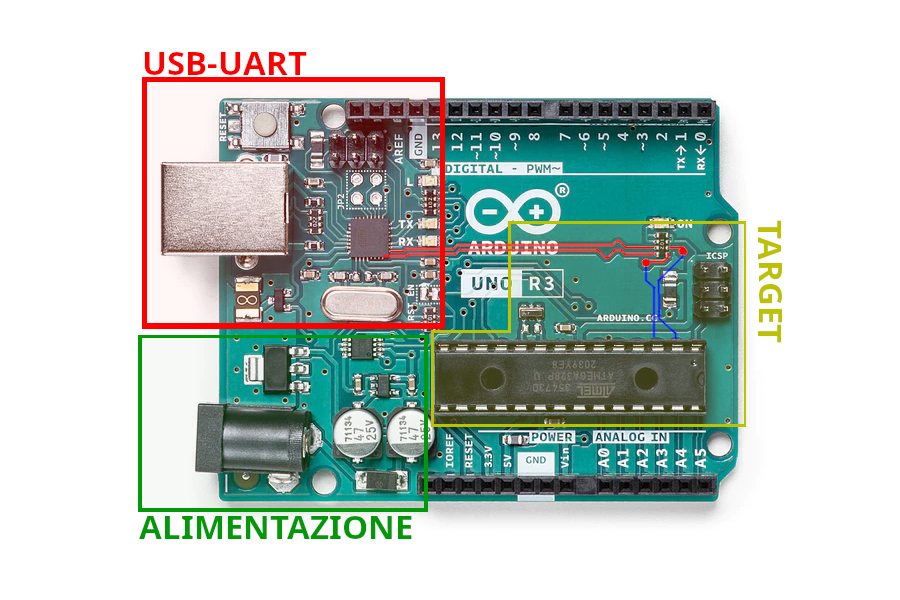
\includegraphics[width=.5\textwidth]{arduino-uno.png}
    \caption[]{Foto di una scheda Arduino Uno R3\cite{img:arduino-uno-r3}}\label{fig:arduino-uno-r3}
\end{figure}

la scheda (Figura~\ref{fig:arduino-uno-r3}) presenta una serie di connettori posti ai lati, collegati ai pin del controllore principale in centro, utili per interconnettere il dispositivo con i circuiti in sviluppo.
L'hardware addizionale presente sul lato sinistro --- invece --- permette di alimentare la scheda da una sorgente esterna non regolata tramite il connettore cilindrico nero e di collegare il controllore principale, tramite connessione seriale, a un computer tramite la porta USB presente in alto a sinistra.
È inoltre possibile effettuare il reset manuale del target tramite il pulsante presente vicino alla presa USB.\@

Il controllore presente al centro della scheda, in un involucro DIP-28\footnote{Dual in-line package, 28 pin}, è un ATMega328P-PU\cite{site:arduino-uno-doc}. È stato scelto un formato così ``datato'' per permettere all'utente di sostituire il chip in caso di guasto.

\section{La famiglia AVR}

Il controllore ATMega328P-PU presente sulla scheda di sviluppo è un membro della famiglia AVR di Atmel\cite{avr:m328p}.

Come è possibile identificare dalla figura~\ref{fig:avr-arch} l'architettura del processore della famiglia AVR è di tipo Harvard: È evidente la dicotomia tra memoria del programma (nell'immagine ``\textit{Flash Program Memory}''), SRAM e EEPROM\cite{harvard-arch}.

La suddivisione consente di ottimizzare separatamente le due diverse tecnologie di storge intrinsecamente diverse.

Come è possibile osservare, la grandezza del bus dati è di 8 bit, di conseguenza è possibile dedurre che l'intera architettura si basa sull'unità fondamentale del byte.

Vi è poi la totale assenza di pipelining essendo un processore a singolo ciclo. La maggior parte delle istruzioni, infatti, viene eseguita in un solo ciclo di clock\cite{avr:m328p} ad esclusione delle operazioni sulle memorie le quali ``stallano'' il processore per questioni di tempi di accesso/scrittura o di istruzioni che involvono dati di lunghezza maggiore di 8 bit.

\begin{figure}[t]
    \centering
    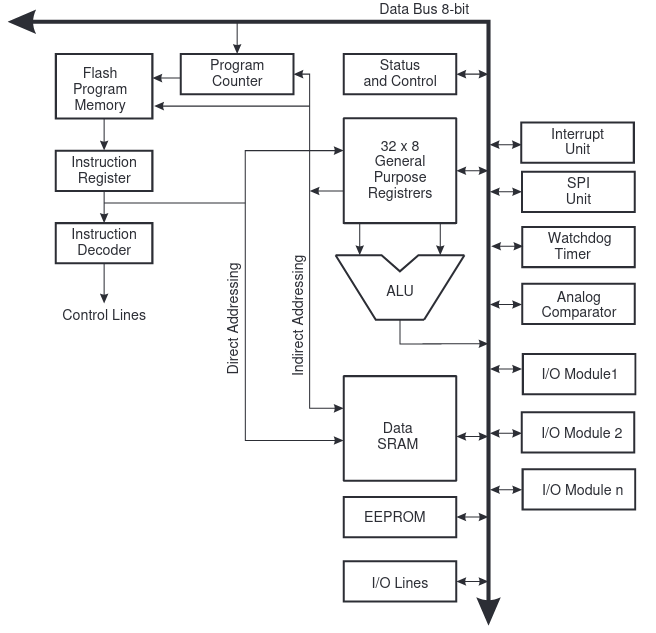
\includegraphics[width=.9\textwidth]{avr_arch.png}
    \caption[Immagine ottenuta dal documento~\cite{avr:m328p}, fig. 7-1]{Schema a blocchi dell'architettura AVR\cite{avr:m328p}}\label{fig:avr-arch}
\end{figure}

\subsection{Funzionalità avanzate}\label{ss:advanced-features}

Infine, per i micro controllori di fascia media, esiste la differenziazione tra codice di bootloader e codice eseguibile.

Il codice ``privilegiato'' è in grado di essere eseguito se si verificano determinati eventi, può essere protetto da sovrascrittura/lettura con criteri diversi dal codice dell'applicazione ed è in grado di riprogrammare la memoria dello stesso integrato mentre è in esecuzione (Read While Write)\cite{avr:m328p}.

\subsection{Memorie}

All'interno di un controllore della famiglia AVR, essendo un processore ad architettura harvard, è possibile trovare due diverse tipologie di memorie dedicate --- utili all'ottimizzazione di costi e funzionamento --- e una terza tipologia tipologia dedicata all'utilità e alla riduzione dei costi dell'hardware.

\subsubsection{Memoria FLASH}
La memoria flash è dedicata alla conservazione del codice eseguibile.
Dato l'utilizzo generale di sola lettura, essa si presenta come una memoria a lettura veloce, organizzata ad unità elementari di 16 bit e riprogrammabile a pagine.

La scelta di indicizzare a ``word'' è stata adottata in quanto la dimensione delle istruzioni dell'\textit{Instruction Set} è sempre di 16 bit oppure, in casi eccezionali, di 32 bit\cite{avr:isa}.

Si tratta poi di una memoria complessa: per i controllori avanzati, aventi il supporto al bootloader, essa è divisa in due sezioni le quali garantiscono la possibilità di differenziare i privilegi del codice presente nelle due sezioni come descritto nella sezione~\ref{ss:advanced-features}.

Essendo poi una memoria ``di programma'', essa non richiede prestazioni notevoli in scrittura: questa avviene quindi a blocchi di 512/1024byte (in funzione del controllore e della dimensione della memoria) e può essere eseguita in due diverse modalità:
\begin{itemize}
    \item ISP\footnote{In System Programming}: In questo caso il controllore è in modalità di programmazione ed esegue i comandi inoltrati da un programmatore esterno --- connesso tramite SPI\footnote{Serial Peripheral Interface} --- mentre la cpu è in stato di \textit{halt}.
    \item Self Programming: Grazie all'istruzione \texttt{spm} è possibile riprogrammare le pagine della memoria flash dall'interno del codice stesso\footnote{Nel caso in cui sia presente il supporto al bootloader, \texttt{spm} può essere eseguito solo se il program counter punta a tale regione.}.
\end{itemize}

\subsubsection{EEPROM}

La memoria EEPROM è considerata una memoria di utilità in quanto non necessariamente essenziale alla vita del codice in esecuzione. Essa permette di salvare dati in modo non volatile nell'eventualità di una mancanza di alimentazione.

Si tratta di una memoria ``lenta'' (tempi di programmazione di 3.3ms~\cite{avr:m328p}) ma in grado di essere letta e scritta con un'unità fondamentale di 8 bit.

Il vantaggio che si presenta con l'integrazione di tale memoria all'interno dell'integrato consiste nell'eliminazione di un ulteriore componente sul circuito stampato nel caso essa sia necessaria, oltre al non utilizzo di una periferica di comunicazione dedicata a tale scopo.

L'interazione con la memoria avviene tramite la scrittura e lettura di determinati registri (\texttt{EECR} \texttt{EEDR} \texttt{EEAR}, EEPROM Control, Data e Address Registers)\cite{avr:m328p}.

\subsubsection{SRAM}
La memoria SRAM è una delle maggiori costituenti della struttura dell'integrato.

Essa consiste nella principale memoria di elaborazione, ma la sua struttura è leggermente più complessa rispetto a quanto si possa trovare su un comune calcolatore.
Infatti l'architettura AVR utilizza in modo marcato il concetto di MMIO\footnote{Memory Mapped Input and Output}.

\begin{figure}[b]
    \centering
    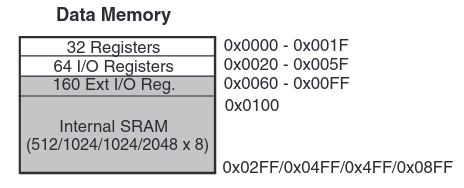
\includegraphics[width=.7\textwidth]{avr_sram_allocation.png}
    \caption[Immagine ottenuta dal documento~\cite{avr:m328p}, fig. 8-3]{Settorizzazione della memoria SRAM del controllore ATMega328P\cite{avr:m328p}}\label{fig:avr-sram-alloc}
\end{figure}

Come è possibile osservare dalla figura~\ref{fig:avr-sram-alloc} i primi 128 byte della memoria SRAM sono in realtà registri di uso generale (\texttt{r0}-\texttt{r31}) o registri di controllo delle periferiche.
La scrittura di tali locazioni di memoria causa effetti collaterali in funzione della periferica alla quale è associata.

È inoltre necessario notare dalla figura~\ref{fig:avr-sram-alloc} come le istruzioni di accesso alla ram impieghino due cicli di clock:l'indicizzazione della ram è effettuata tramite un indirizzamento di 16 bit, il quale rende necessario l'utilizzo congiunto di due registri (r26-r27, r28-r29, r30-r31). 

Questa operazione infatti consente di calcolare l'indirizzo al quale effettuare l'operazione incrementando, decrementando oppure lasciando invariata la coppia di registri di indicizzazione pre o post esecuzione.

\begin{figure}[t]
    \centering
    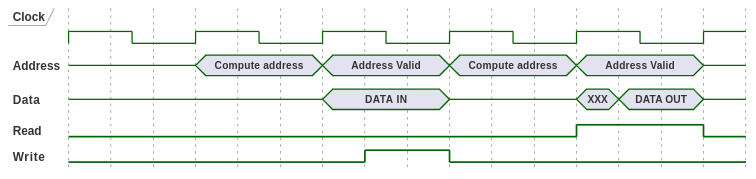
\includegraphics[width=.9\textwidth]{sram-access-timings.png}
    \caption[Immagine rielaborata a partire dalla fig. 8-4 del documento~\cite{avr:m328p}]{Sequenze di accesso in lettura e scrittura della memoria SRAM\cite{avr:m328p}}\label{fig:avr-sram-timings}
\end{figure}

in particolare, un uso comune delle istruzioni di accesso alla memoria viene mostrato dal listato \ref{}

\begin{lstlisting}[language=AVR, caption={Esempio}]
    st r24, X+
\end{lstlisting}

\section{Il protocollo DebugWire}
\subsection{Funzionamento}
\subsection{Comandi e features}